
\chapter{Core Classes}\label{coreclasses}
\pagecolor{gray}\afterpage{\nopagecolor}
\newpage
\pagecolor{gray}\afterpage{\nopagecolor}
\fontfamily{pzc}
\selectfont
Co-Consul of Ablon enters the Office and the General Autorius sits at his table, golden goblets of wine and a plate full of grapes rests easy in front of him. 

``We had an agreement, that we'd share all revenue.''

``Yes''

``Hereopolis has agreed to give you 20,000 pounds of gold. I want my share.''

``Who told you this?''

``You deny?''

``Who told him.''

``I have spies among his people.''

``If Herod is kind enough to give me a gift, what business is it of yours? A gift is not revenue.''

It is not a gift, it is a bribe. For political and military favours. The cost of which favours shall be born by the state.''

``Peasantry.''

``Let us be realistic. This arrangement of ours can not work if you seek every opportunity to aggrandize yourself at my expense.''

``Laughter. Aggrandize myself. This from the boy whose so called father has been declared a God.''

``An honour he well deserves.''

``You only did it so you might be known as the Son of a God. You have no accomplishments of your own, so you seek to borrow the glory of others.''

``Its true, it was no accomplishment to defeat you at Mutina.''

``You defeated me? You cowardly little shit. You never left your tent. You have never defeated me, in anything.''

``Gentlemen, lets not get overheated. Im sure we can come to some reasonable agreement. I had hoped that you had learnt some humility and discipline. You are still the same old crude, arrogant, lech that you always were.''

``Thats right. Just the same. The same that is still fucking your mother!''
\normalfont
\newpage

%changing the page design temporarily
\changepage{9cm}{9.4cm}{-4.7cm}{-4.7cm}{}{-4.5cm}{}{}{}
%\noindent\rule{\textwidth}{\textheight}
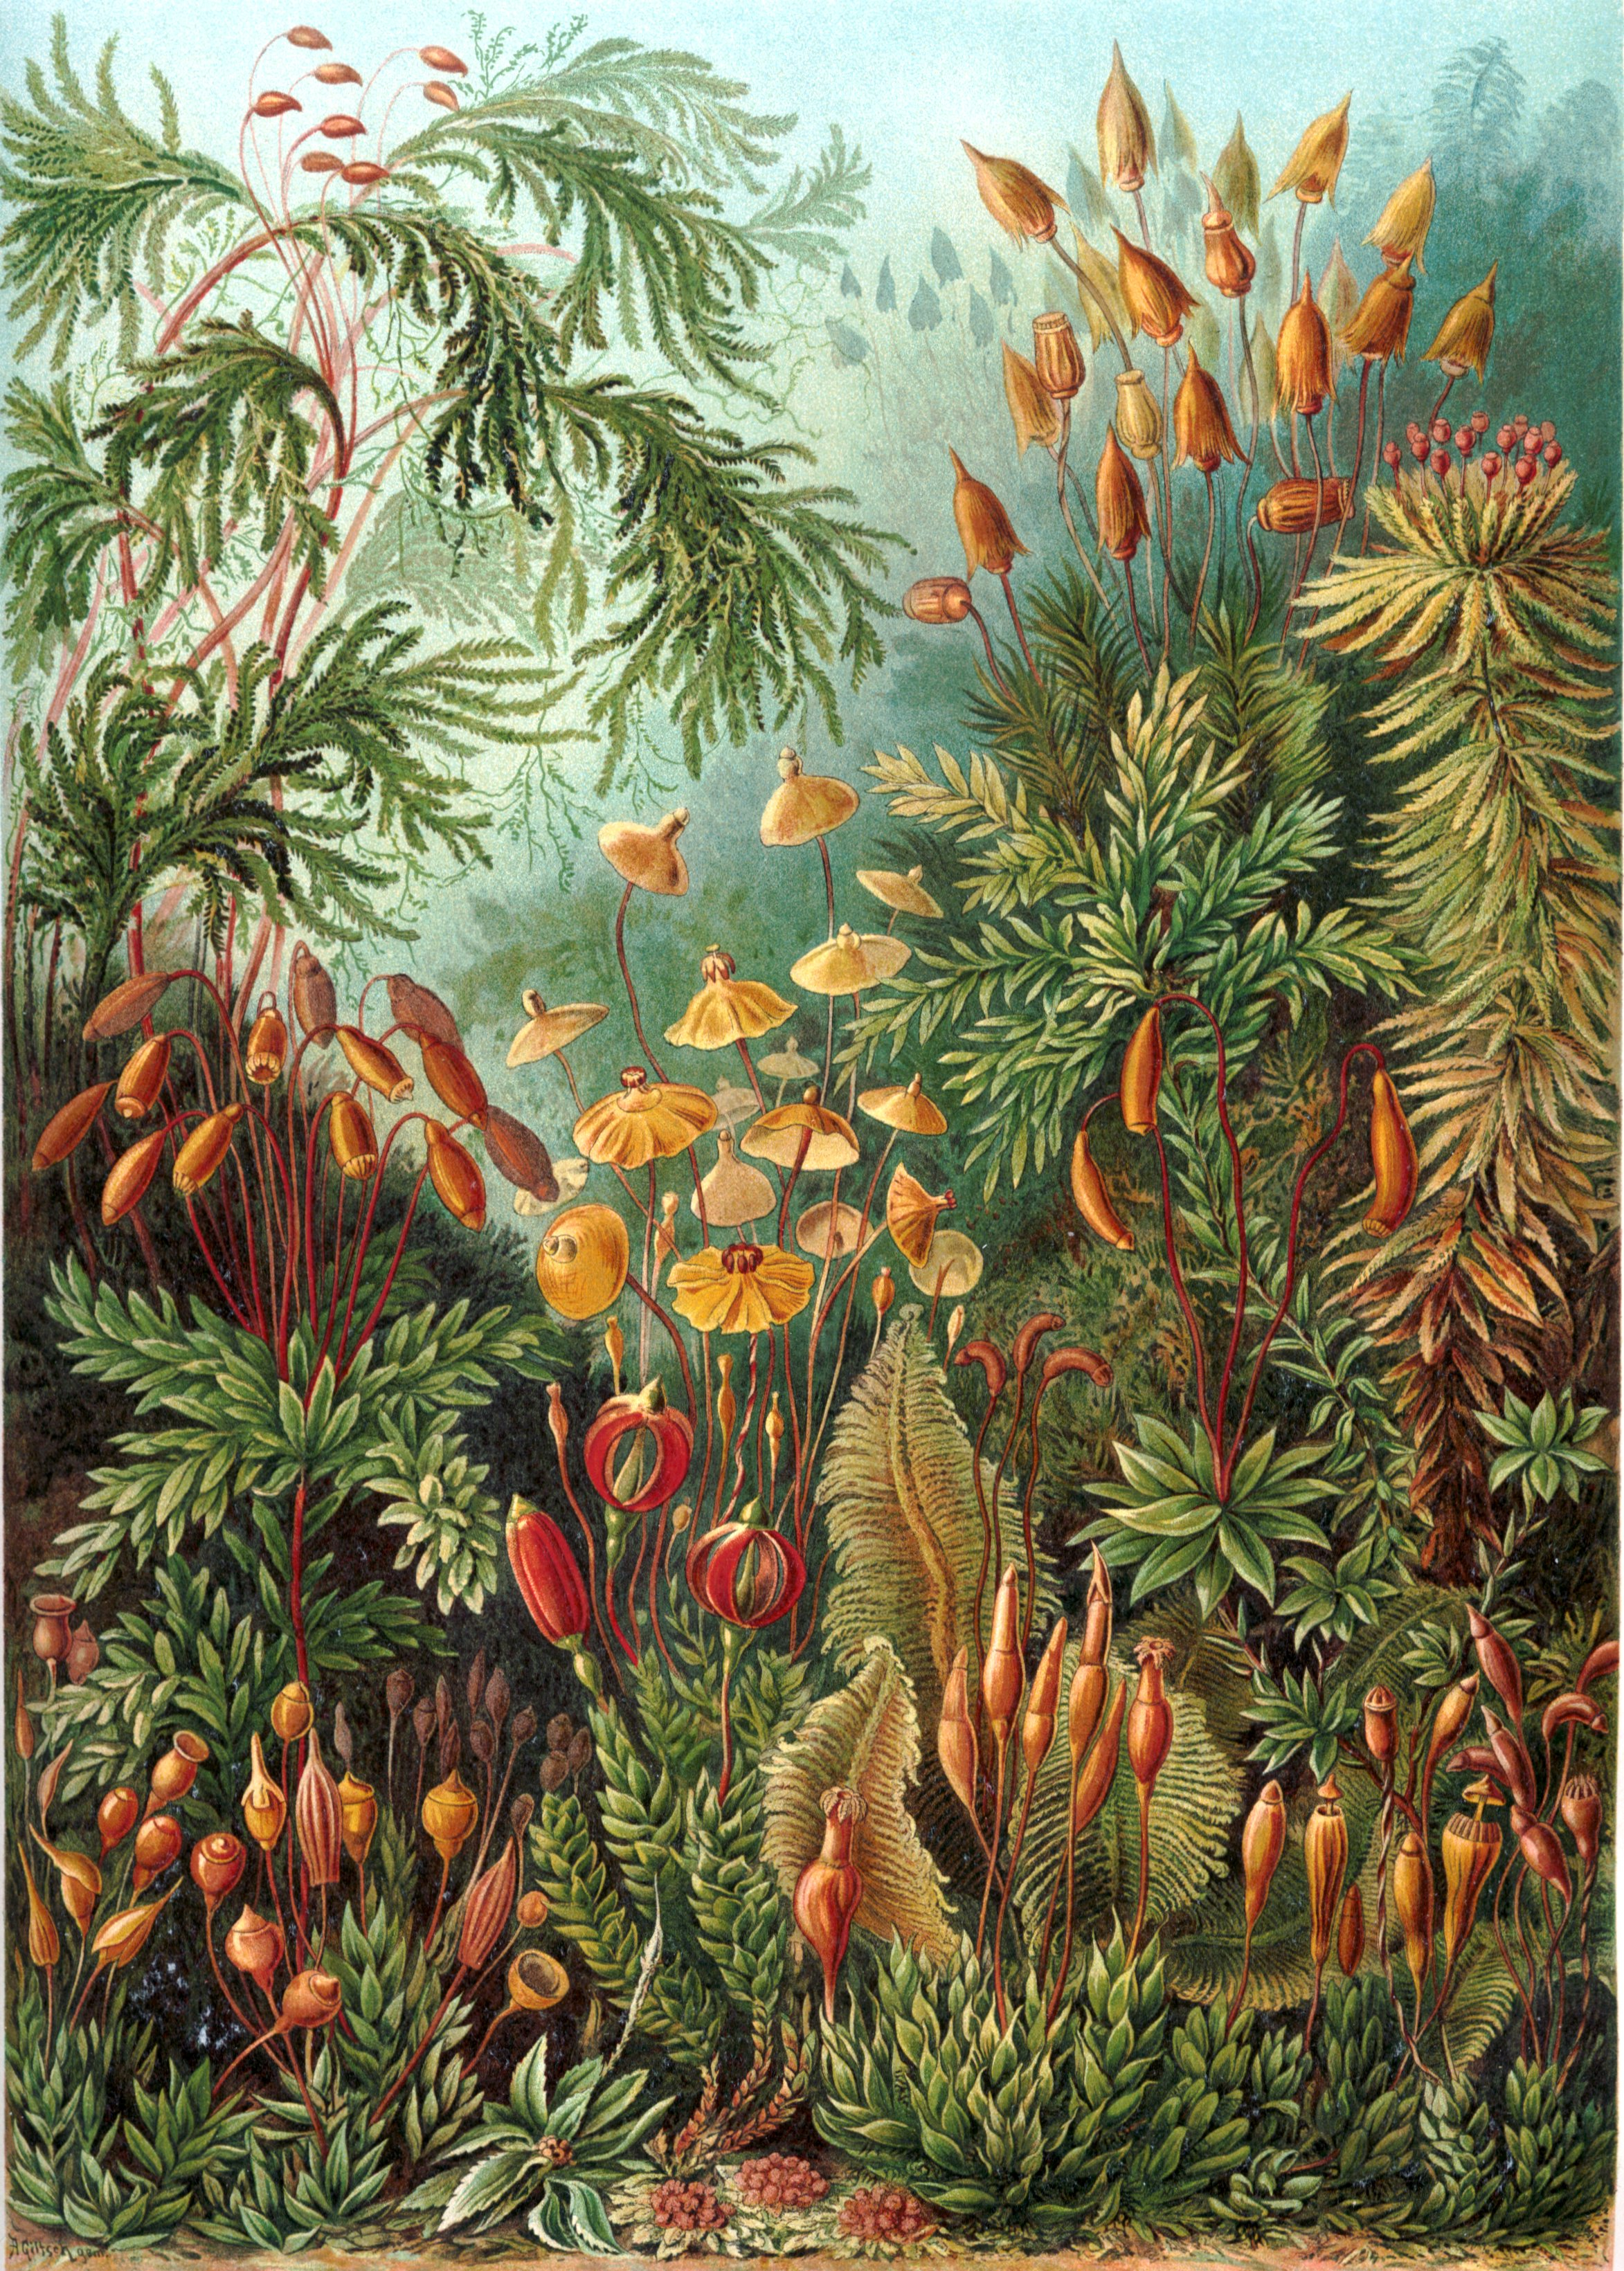
\includegraphics[width=\textwidth,height=\textheight]{Haeckel_Muscinae}
\newpage

%restoring the standard settings
\changepage{-9cm}{-9.4cm}{4.7cm}{4.7cm}{}{4.5cm}{}{}{}

\begin{multicols}{2}
The Core Classes are archetypical classes to the worlds most popular RPG system. They encapsulate problem solving philosophies and a way of playing the game. 

This class system is designed to be extremely simple. It is fundamentally an "open formed gaming" system. I.e. pretty much every character can sneak around, or swim, or climb walls. The difference is that certain characters have additional capabilities above the norm. 

It is very fine to have an entire party composed of Fighters. Having a cleric on the team greatly increases survivability however. 

\section{Fighter} This class is best at solving problems via brute force. They are not just a duelist but are skilled in any form of warfare. 

The Fighter may use any weapon or armour. Their starting HP is 10. Each time they level up they must roll 1d10 to determine the HP gained for that level up. This makes them a very tough class to kill relative to the other classes.

The Fighter class is illiterate but can speak in Common.  

\section{Wizard} They are the late game class. Their starting HP is 4, and they gain 1d4 hp per level up. Most wizards are proficient with no weapons and armour, unless some other mechanic such as Race dictates otherwise. To survive you will have to master using terrain and keeping aware of your surroundings. 

The capabilities of the Wizard are virtually unknown. They are an esoteric class whom start off as a Scholar without spellcasting capabilities and must learn dark secrets to unlock their potential. They are thus not suitable for brief adventures and best suited for campaign play.

As a Wizard you begin knowledgeable in one of the fields of Academia. You have two basic ways to use this. You can ask the GM for advice or information pertaining to the topic, and/or you can use your own knowledge of the topic (relevant to the time period of the game) to your own advantage. 

The Wizard class begins literate in Common and High Common - the language of the nobility classes.  
 
\section{Rogue} Rogues may only wear leather armour and are severely limited in their weapon selection. The most common rogue weapons are Daggers and Shortbows. Their starting HP is 4 and they roll 1d4 each time they level up for extra HP. The rogue class has access to a number of special skills that provides them additional utility. 

Their two principal combat abilities are Backstab and Set Traps. Their utility abilities are: Hide in Shadows, Climb Steep Slopes, and Listen at Doors.

The Rogue class is illiterate but can speak in both Common and Low Common - the language of the criminal underworld. 

\section{Cleric}

Clerics may wear armour and use any weapon. Their starting HP is 8 and they roll 1d8 each time they level up for extra HP. 

The principal advantage of playing a Cleric is that of your involvement with society at large. If you have a local congregation, it is likely that they will come to your aid, and it is expected that you come to theirs in times of need. 

Some Churches become extremely powerful allies. Also, ostensibly, merchants are less willing to rip off Clerics than other classes. This is not a fool proof way of being safe from scams however.  

The Cleric class can read and write in Common and Gothic - an ancient language of religious scripture.

\end{multicols}
